\documentclass[pointlessnumbers, abstracton, headsepline, a4paper]{scrartcl}

\usepackage[T1]{fontenc}
\usepackage[utf8]{inputenc}
\usepackage{graphicx}
\usepackage{microtype}
\usepackage{textcomp}
\usepackage{ellipsis, fixltx2e, mparhack, booktabs, longtable}
\usepackage[automark]{scrpage2}
\usepackage{multicol}
\usepackage{microtype}
\usepackage{listings}
\usepackage[a4paper]{geometry}
\usepackage[polish]{babel}
\usepackage{subfigure}
\usepackage{tikz}
\usetikzlibrary{arrows,positioning}

\usepackage{courier}
\lstset{
         basicstyle=\footnotesize\ttfamily, % Standardschrift
         %numbers=left,               % Ort der Zeilennummern
         numberstyle=\tiny,          % Stil der Zeilennummern
         %stepnumber=2,               % Abstand zwischen den Zeilennummern
         numbersep=5pt,              % Abstand der Nummern zum Text
         tabsize=2,                  % Groesse von Tabs
         extendedchars=true,         %
         breaklines=true,            % Zeilen werden Umgebrochen
         keywordstyle=\color{red},
         stringstyle=\color{white}\ttfamily, % Farbe der String
         showspaces=false,           % Leerzeichen anzeigen ?
         showtabs=false,             % Tabs anzeigen ?
         showstringspaces=false      % Leerzeichen in Strings anzeigen ?        
}

% part of the hyperref bundle
\usepackage{ifpdf}

\geometry{verbose,tmargin=3.5cm,bmargin=3.5cm}
\setlength{\parskip}{\medskipamount}
\setlength{\parindent}{0pt}

\clearscrheadfoot
\ohead{\\\headmark}
\ihead{
\includegraphics[scale=0.2]{img/zut2.jpg}}
\ofoot[\pagemark]{\pagemark}

% if pdflatex is used
\ifpdf

%set fonts for nicer pdf view
\IfFileExists{lmodern.sty}{\usepackage{lmodern}}
  {\usepackage[scaled=0.92]{helvet}
    \usepackage{mathptmx}
    \usepackage{courier} }
\fi

% the pages of the TOC are numbered roman
% and a pdf-bookmark for the TOC is added
\pagenumbering{arabic}
\let\myTOC\tableofcontents
\renewcommand\tableofcontents{\myTOC\clearpage\pagenumbering{arabic}}

\begin{document}
\begin{titlepage}

\begin{center}

\includegraphics[scale=0.5]{logos/zut.jpg}
\par
\end{center}

\begin{center}
\textsf{\textbf{\LARGE Wydział Informatyki}}
\end{center}{\LARGE}

\vspace{1.5cm}

\begin{center}
\textsf{\Large Metody sztucznej inteligencji}
\end{center}

\begin{center}
\textsf{\textbf{\Large Laboratorium 03 IUz-22 Urbaniak}}
\end{center}

\begin{center}
\textsf{\large Sprawozdanie}
\end{center}

\vspace{3.5cm}

\begin{center}
\begin{tabular}{ll}
Autor: & Sergiusz Urbaniak\tabularnewline
Grupa: & IUz-22\tabularnewline
Data: & \today\tabularnewline
\end{tabular}
\end{center}

\end{titlepage}

\tableofcontents

\section{Badania plików}
W następujących oddziałach są pokazane wyniki uczenia konkurencyjnego podanych plików. Najpierw w tabeli są przedstawione neurony i ich uczone wagi. Potem jest pokazany wynik uczenia.

\subsection{\texttt{dane1.txt}}

\begin{table}[h]
\centering
\begin{tabular}[t]{c|c}
Neuron & Wagi \\
\hline
1 & 0.8566,  -0.0946 \\
2 &-0.7966,   0.3138 \\
3 &-0.0100,  -0.1565 \\
4 & 0.0753,  -0.8150 \\
\end{tabular}
\caption{\label{tab:xor}Wagi uczonych neuronów pliku \texttt{dane1.txt}}
\end{table}

\begin{figure}[!h]
\centering
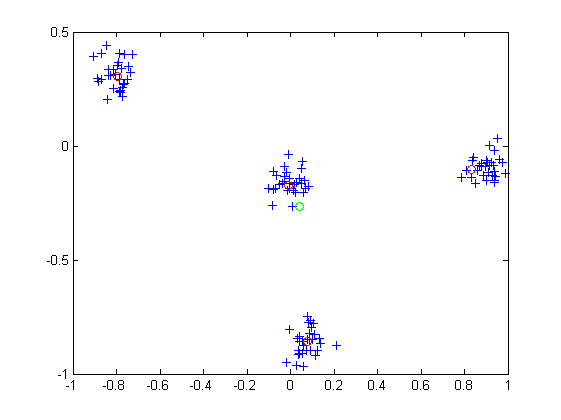
\includegraphics[scale=0.8]{src/dane1.png}\caption{\label{fig:dane1}Wyniki uczenia}
\end{figure}

\clearpage
\subsection{\texttt{dane2.txt}}

\begin{table}[h]
\centering
\begin{tabular}[t]{c|c}
Neuron & Wagi \\
\hline
1&  0.4372,  -0.6343 \\
2& -0.3693,  -0.2767 \\
3&  0.4129,   0.9439 \\
4& -0.2477,   0.4151 \\
5&  0.6246,  -0.0639 \\
\end{tabular}
\caption{\label{tab:xor}Wagi uczonych neuronów pliku \texttt{dane2.txt}}
\end{table}

\begin{figure}[!h]
\centering
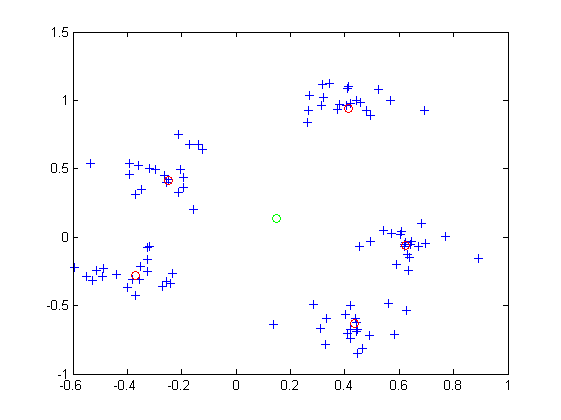
\includegraphics[scale=0.8]{src/dane2.png}\caption{\label{fig:dane1}Wyniki uczenia}
\end{figure}

\clearpage
\subsection{\texttt{dane3.txt}}

\begin{table}[h]
\centering
\begin{tabular}[t]{c|c}
Neuron & Wagi \\
\hline
1&  0.3999,  -0.4940 \\
2& -0.4454,  -0.2632 \\
3& -1.0240,  -0.1175 \\
4&  0.8445,  -0.1047 \\
5&  0.3707,   0.4891 \\
\end{tabular}
\caption{\label{tab:xor}Wagi uczonych neuronów pliku \texttt{dane3.txt}}
\end{table}

\begin{figure}[!h]
\centering
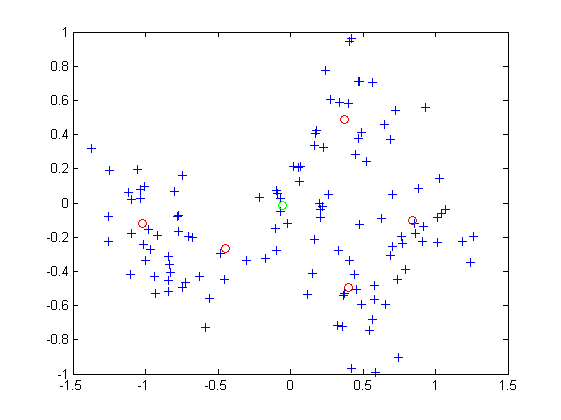
\includegraphics[scale=0.8]{src/dane3.png}\caption{\label{fig:dane1}Wyniki uczenia}
\end{figure}

\clearpage
\subsection{\texttt{dane3d1.txt}}

\begin{table}[h]
\centering
\begin{tabular}[t]{c|c}
Neuron & Wagi \\
\hline
1& -0.2860,  -0.0676,   0.1099 \\
2&  0.1101,  -0.0131,   0.2516 \\
3& -0.1527,   0.1315,   0.1206 \\
4& -0.0069,   0.1796,   0.2781 \\
\end{tabular}
\caption{\label{tab:xor}Wagi uczonych neuronów pliku \texttt{dane3d1.txt}}
\end{table}

\begin{figure}[!h]
\centering
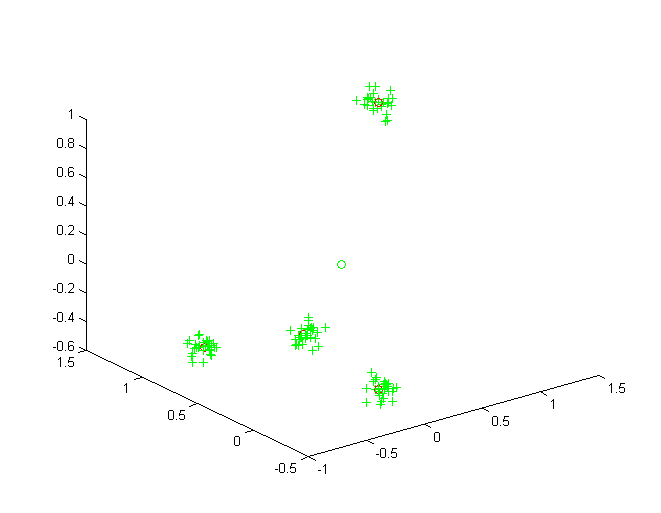
\includegraphics[scale=0.8]{src/dane3d1.png}\caption{\label{fig:dane1}Wyniki uczenia}
\end{figure}

\clearpage
\subsection{\texttt{dane3d2.txt}}

\begin{table}[h]
\centering
\begin{tabular}[t]{c|c}
Neuron & Wagi \\
\hline
1&  0.2261,   0.7919,   0.9134 \\
2& -0.7728,   0.6324,  -0.5033 \\
3& -0.8225,  -0.4064,   0.2913 \\
4&  0.9081,  -0.2220,   0.6549 \\
5& -0.9577,  -0.7378,  -0.1668 \\
\end{tabular}
\caption{\label{tab:xor}Wagi uczonych neuronów pliku \texttt{dane3d2.txt}}
\end{table}

\begin{figure}[!h]
\centering
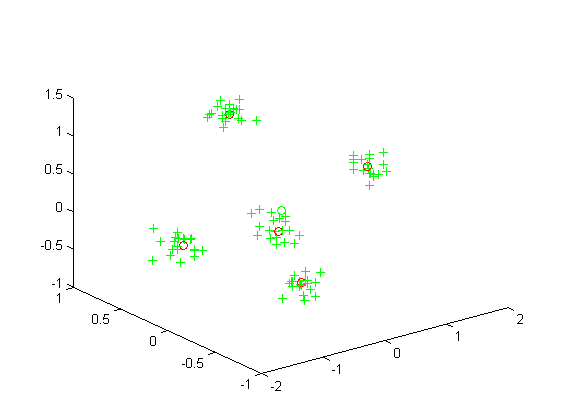
\includegraphics[scale=0.8]{src/dane3d2.png}\caption{\label{fig:dane1}Wyniki uczenia}
\end{figure}

\clearpage
\subsection{\texttt{dane3d3.txt}}

\begin{table}[h]
\centering
\begin{tabular}[t]{c|c}
Neuron & Wagi \\
\hline
1&  0.3386,  -0.3440,  -0.7325 \\
2& -0.2812,   0.7484,   0.3229 \\
3& -0.3490,  -0.7794,  -0.4610 \\
4& -0.7397,  -0.0117,  -0.2279 \\
\end{tabular}
\caption{\label{tab:xor}Wagi uczonych neuronów pliku \texttt{dane3d3.txt}}
\end{table}

\begin{figure}[!h]
\centering
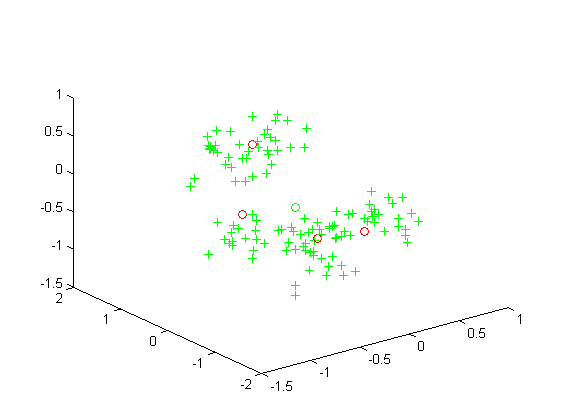
\includegraphics[scale=0.8]{src/dane3d3.png}\caption{\label{fig:dane1}Wyniki uczenia}
\end{figure}

\clearpage
\subsection{\texttt{kapitan\_i.txt}}

\begin{table}[h]
\centering
\begin{tabular}[t]{c|c}
Neuron & Wagi \\
\hline
1& 38.8117,  -0.5899,  -7.1230 \\
2&-43.3287,   0.8705,   8.1441 \\
3&  6.4899,   0.2057,   2.1501 \\
4&-14.0384,  -2.8818,  -1.9704 \\
\end{tabular}
\caption{\label{tab:xor}Wagi uczonych neuronów pliku \texttt{kapitan\_i.txt}}
\end{table}

\begin{figure}[!h]
\centering
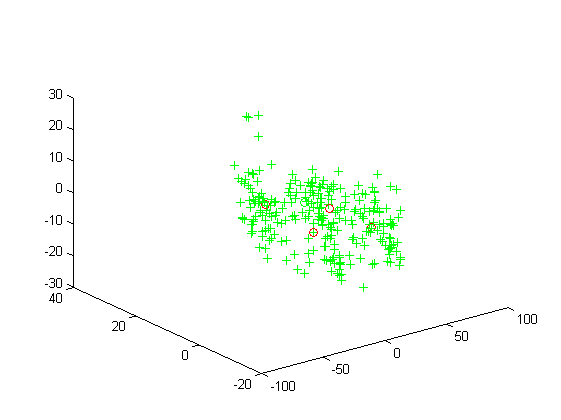
\includegraphics[scale=0.8]{src/kapitan_i.png}\caption{\label{fig:dane1}Wyniki uczenia}
\end{figure}

\clearpage
\section{Własna funkcja uczenia konkurencyjnego}
\subsection{Wzory}

Przy uczeniu konkurencyjnym neurony nie posiadają funkcji aktywacji. Wejścia neuronów bezpośrednio są przeliczane za pomocą wag według wzoru \ref{eq:weights}.

\begin{equation}
\label{eq:weights}
y_n = W^T_n X = \sum_{i=1}^{n} w_{i,n} \, x_i
\end{equation}

\begin{figure}[!h]
\centering
\def\layersep{2.5cm}

% Define two helper counters
\begin{tikzpicture}[shorten >=1pt,->,draw=black, node distance=\layersep]
    \tikzstyle{every pin}=[pin distance=\layersep/2]
    \tikzstyle{every pin edge}=[pin edge={->}, shorten <=1pt]
    \tikzstyle{neuron}=[circle,fill=black!25,minimum size=20pt,inner sep=0pt]
    \tikzstyle{annot} = [text width=4em, text centered]

    % Draw the input layer nodes
    \foreach \name / \x in {1,...,2}
        \node (I-\name) at (0,-\x*2-1) {$x_\x$};

    \foreach \name / \y in {1,...,3}
        \path
            node [neuron, pin={right:$y_\y$}, label={above:
$W_\y=\left(\begin{array}{c}w_{1,\y} \\ w_{2,\y} \end{array}\right)$
		}] (H-\name) at (\layersep*1.5,-\y*2 cm) {$\Sigma$};

    % Connect every node in the input layer with every node in the
    % hidden layer.
    \foreach \source in {1,...,2}
        \foreach \dest in {1,...,3}
            \path (I-\source) edge (H-\dest);
\end{tikzpicture}

\caption{\label{fig:distance}Sieć neuronów konkurencyjnych}
\end{figure}

Wagi $W_n$ danej iteracji są korygowane tylko dla tego neuronu, który najmocniej zostaje pobudzony. Pobudzenie jest mierzone odległością między neuronem a punktem wejściowym wektorem $d$ według wzoru \ref{eq:distance}.

\begin{equation}
\label{eq:distance}
\begin{array}{rclc}
\vec d & = & \vec x-\vec w_k & \textrm{gdzie odległośc jest} \\
|\vec d| & = & \sqrt{(w_1-x_1)^2+(w_2-x_2)^2+\ldots+(w_n-x_n)^2} &
\end{array}
\end{equation}

\begin{figure}[!h]
\centering
\def\layersep{2.5cm}

\begin{tikzpicture}
	\filldraw
		[blue] (0,4) circle (2pt);

	\filldraw
		[red] (5,4) circle (2pt);

	\filldraw
		[red] (3,4) circle (2pt);

	\draw [thick,-angle 90] (0,0) -- node[anchor=east] {$\vec x$} (0,4);

	\draw [thick,-angle 90] (0,0) -- node[anchor=east] {$\vec w_{k+1}$} (3,4);

	\draw [thick,-angle 90] (0,0) -- node[anchor=east] {$\vec w_k$} (5,4);

	\draw [-angle 90, green] (5,4) -- (0,4) node[black, anchor=south] {$\vec d=\vec x- \vec w_k$};

	\draw [very thick, -angle 90, orange] (5,4) -- node[black, anchor=south] {$\Delta w = \eta(\vec x-\vec w_k)$} (3,4);
\end{tikzpicture}

\caption{\label{fig:distance}Wektorowa reprezentacja iteracji uczenia}
\end{figure}

Największe pobudzenie jest wtedy osiągane jeżeli znajdziemy neuron z najmniejszą odległością $|\vec d|_{min}$ dla danej iteracji. Wtedy korygowane są wagi $W_{k+1}$ danego neuronu według wzoru \ref{eq:delta}.

\begin{equation}
\label{eq:delta}
\begin{array}{rclc}
W_{k+1} & = & \Delta w + W_k & \textrm{gdzie} \\
\Delta w & = & \eta(X-W_k)
\end{array}
\end{equation}

W następnym rozdziale są przedstawiane wyniki badan z zaimplementowanym algorytmem. Kod algorytmu jest widoczny w listingu \ref{lst:nadzor} w rozdziale \ref{sec:nadzor}. Tradycyjnie kod został napisany w Octave pod systemem Linux.

\clearpage
\subsection{\texttt{dane1.txt}}

\begin{table}[h]
\centering
\begin{tabular}[t]{c|c}
Neuron & Wagi \\
\hline
1 &   0.042189, -0.835570 \\
2 &   0.927179, -0.130506 \\
3 &  -0.866712,  0.290581 \\
4 &  -0.078092, -0.111721 \\
\end{tabular}
\caption{\label{tab:xor}Wagi uczonych neuronów pliku \texttt{dane1.txt}}
\end{table}

\begin{figure}[!h]
\centering
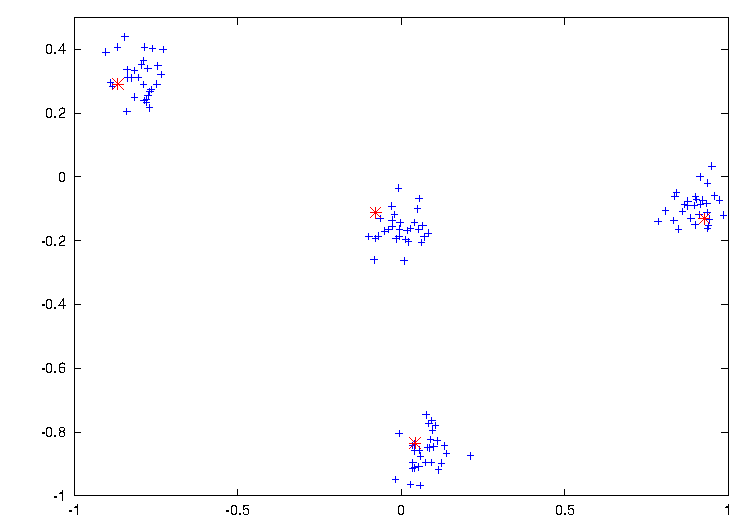
\includegraphics[scale=1.0]{src/mydane1.pdf}\caption{\label{fig:dane1}Wyniki uczenia}
\end{figure}

\clearpage
\subsection{\texttt{dane2.txt}}

\begin{table}[h]
\centering
\begin{tabular}[t]{c|c}
Neuron & Wagi \\
\hline
1& 0.4753834,  0.9282058 \\
2&-0.3521456, -0.2996429 \\
3&-0.3582966,  0.5332628 \\
4& 0.7693442,  0.0098722 \\
5& 0.4220855, -0.6704579 \\
\end{tabular}
\caption{\label{tab:xor}Wagi uczonych neuronów pliku \texttt{dane2.txt}}
\end{table}

\begin{figure}[!h]
\centering
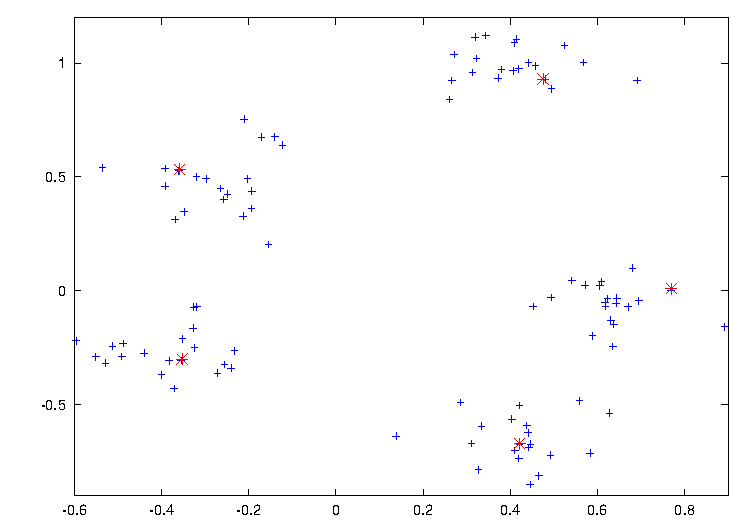
\includegraphics[scale=1.0]{src/mydane2.pdf}\caption{\label{fig:dane1}Wyniki uczenia}
\end{figure}

\clearpage
\subsection{\texttt{dane3.txt}}

\begin{table}[h]
\centering
\begin{tabular}[t]{c|c}
Neuron & Wagi \\
\hline
1&   0.33542,  -0.71606 \\
2&  -0.84005,  -0.35707 \\
3&   0.24094,   0.76322 \\
4&   0.76744,  -0.19235 \\
\end{tabular}
\caption{\label{tab:xor}Wagi uczonych neuronów pliku \texttt{dane3.txt}}
\end{table}

\begin{figure}[!h]
\centering
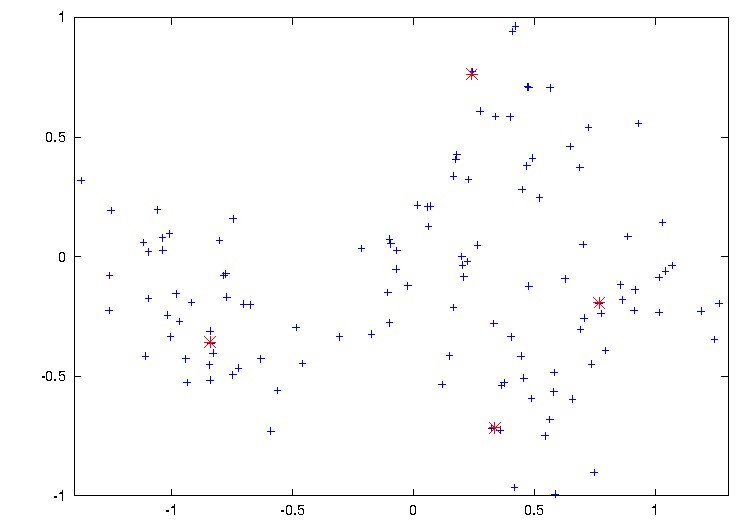
\includegraphics[scale=1.0]{src/mydane3.pdf}\caption{\label{fig:dane1}Wyniki uczenia}
\end{figure}

\clearpage
\subsection{\texttt{dane3d1.txt}}

\begin{table}[h]
\centering
\begin{tabular}[t]{c|c}
Neuron & Wagi \\
\hline
1&  -0.878974,  -0.309702,   0.133947 \\
2&  -0.013616,  -0.107567,  -0.480594 \\
3&   0.932130,   0.973650,   0.971466 \\
4&  -0.723387,   0.691054,  -0.337821 \\
\end{tabular}
\caption{\label{tab:xor}Wagi uczonych neuronów pliku \texttt{dane3d1.txt}}
\end{table}

\begin{figure}[!h]
\centering
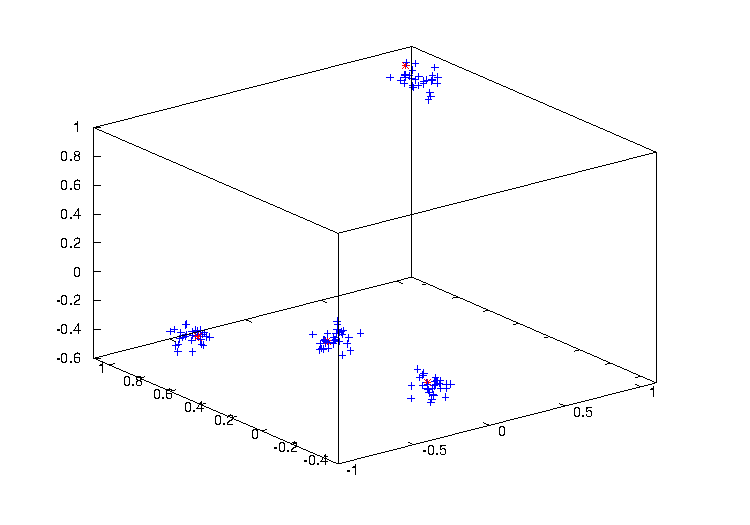
\includegraphics[scale=1.0]{src/mydane3d1.pdf}\caption{\label{fig:dane1}Wyniki uczenia}
\end{figure}

\clearpage
\subsection{\texttt{dane3d2.txt}}

\begin{table}[h]
\centering
\begin{tabular}[t]{c|c}
Neuron & Wagi \\
\hline
1&   0.80463,  -0.14690,   0.55540 \\
2&  -0.90488,  -0.80573,  -0.11126 \\
3&   0.19803,   0.63894,   0.92120 \\
4&  -0.52862,   0.76973,  -0.52255 \\
5&   0.36165,   0.88769,  -0.72851 \\
\end{tabular}
\caption{\label{tab:xor}Wagi uczonych neuronów pliku \texttt{dane3d2.txt}}
\end{table}

\begin{figure}[!h]
\centering
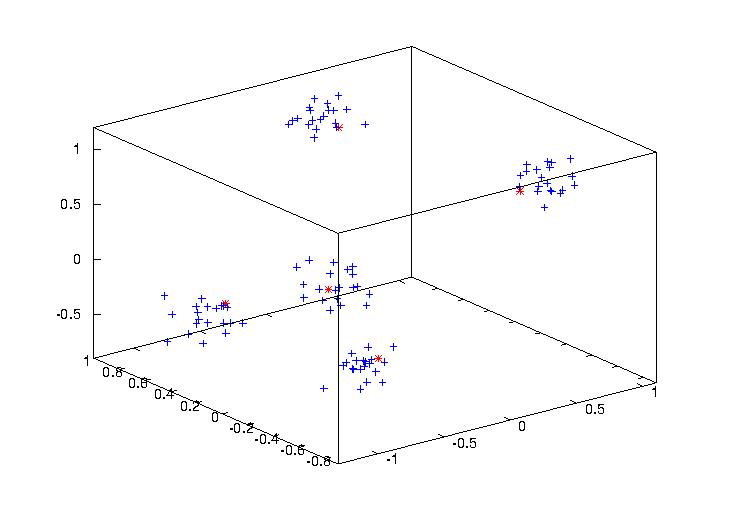
\includegraphics[scale=1.0]{src/mydane3d2.pdf}\caption{\label{fig:dane1}Wyniki uczenia}
\end{figure}

\clearpage
\subsection{\texttt{dane3d3.txt}}

\begin{table}[h]
\centering
\begin{tabular}[t]{c|c}
Neuron & Wagi \\
\hline
1&  -0.55551,   0.89028,   0.34978 \\
2&  -0.42394,  -0.24565,  -0.70310 \\
3&  -0.74934,  -1.03103,  -0.30708 \\
4&   0.61840,  -0.21862,  -0.41426 \\
\end{tabular}
\caption{\label{tab:xor}Wagi uczonych neuronów pliku \texttt{dane3d3.txt}}
\end{table}

\begin{figure}[!h]
\centering
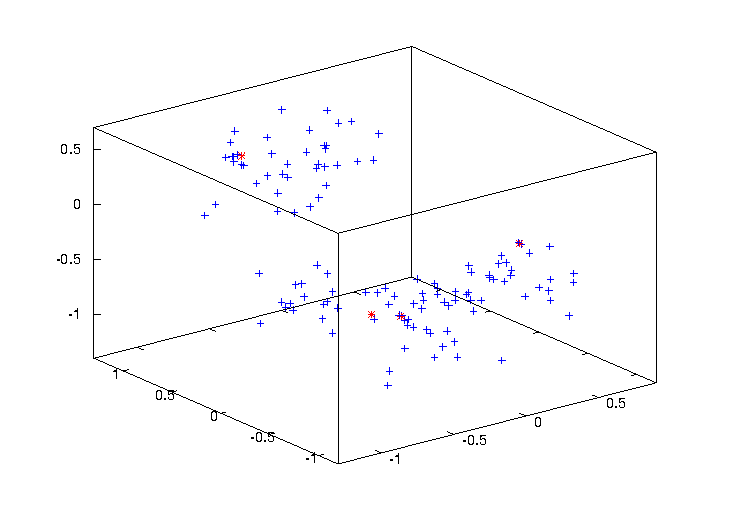
\includegraphics[scale=1.0]{src/mydane3d3.pdf}\caption{\label{fig:dane1}Wyniki uczenia}
\end{figure}


\clearpage
\subsection{\texttt{kapitan\_i.txt}}

\begin{table}[h]
\centering
\begin{tabular}[t]{c|c}
Neuron & Wagi \\
\hline
1&  -28.56914,    6.30167,  -12.52388 \\
2&   -5.16547,   -7.86742,  -11.05208 \\
3&   46.48602,    6.37457,  -19.95036 \\
4&   34.82169,   10.80715,  -15.72390 \\
5&    0.24909,    0.91634,    6.73213 \\
\end{tabular}
\caption{\label{tab:xor}Wagi uczonych neuronów pliku \texttt{kapitan\_i.txt}}
\end{table}

\begin{figure}[!h]
\centering
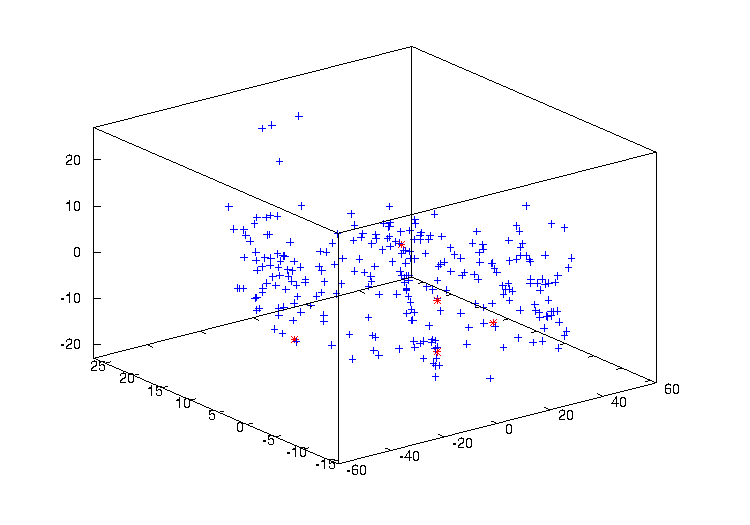
\includegraphics[scale=1.0]{src/mykapitan_i.pdf}\caption{\label{fig:dane1}Wyniki uczenia}
\end{figure}

\clearpage
\subsection{Kod uczenia \texttt{nadzor.m}}
\label{sec:nadzor}
\begin{center}
\lstset{captionpos=b,caption=Kod uczenia konkurencyjnego,label=lst:nadzor}
\lstinputlisting{src/nadzor.m}
\end{center}

\end{document}
